\section{EVALUATION }
\label{section:results}

\subsection{Simulation}
To verify our method and obtain an intuitive understanding of the localization performance under different conditions,
we developed a Monte Carlo simulator that implements
both SBL and HPI-SBL using MATLAB. 
In the simulation, we randomly deployed some smartphones (default 20) in a $10m \times 10m$ area. 
Considering the impact of the uncertainty of node position and TOA detection, we added a certain amount of node location error (default 0.4m) and TOA measurement error (default 2ms) in all the simulations.
Table 1 lists default configurations of major parameters in the simulation.
All statistics reported are RMSE  over 100 trial runs for high confidence. The results of simulation evaluation are as follows.


\begin{table} \normalsize
\caption {\textbf{Default configuration parameter}} %title of the table
\centering % centering table
    \begin{tabular}{|c|c|}
        \hline
\textbf{Parameter} & \textbf{Description} \\
 \hline
Field Area & 10m $\times$10m \\
\hline
Number of Anchors & 20 (Default) \\
 \hline
Node Location Error 	 & 0.4m (Default) \\
 \hline
TOA Detection Error 	 & 2ms (Default) \\
 \hline
Random-Seed Loop	 & 500 times (Default) \\
% \hline
%Error Statistics	 &  RMSE \\
        \hline
    \end{tabular}
\end{table}


\textbf{1) Impact of the number of anchors:}
 In this experiment, we investigated the localization error and number of anchors with a different number of anchors from 10 to 40 in steps of 3. 
 TOA error is 2ms, and other simulation parameters are default values.
With more anchors, the whole space area will be divided into smaller parts, thus more accurate localization estimation could be achieved. 
The results shown in Fig.\ref{fig4} indicates that, as the number of anchor nodes increases, the localization error decreases for both methods.
Fig.\ref{fig4} shows that the localization error of HPI-SBL method is smaller than the SBL method.

 \begin{figure}[htb]
            \setlength{\abovecaptionskip}{0pt}
            \centering
			 \vspace{-2mm}
           		 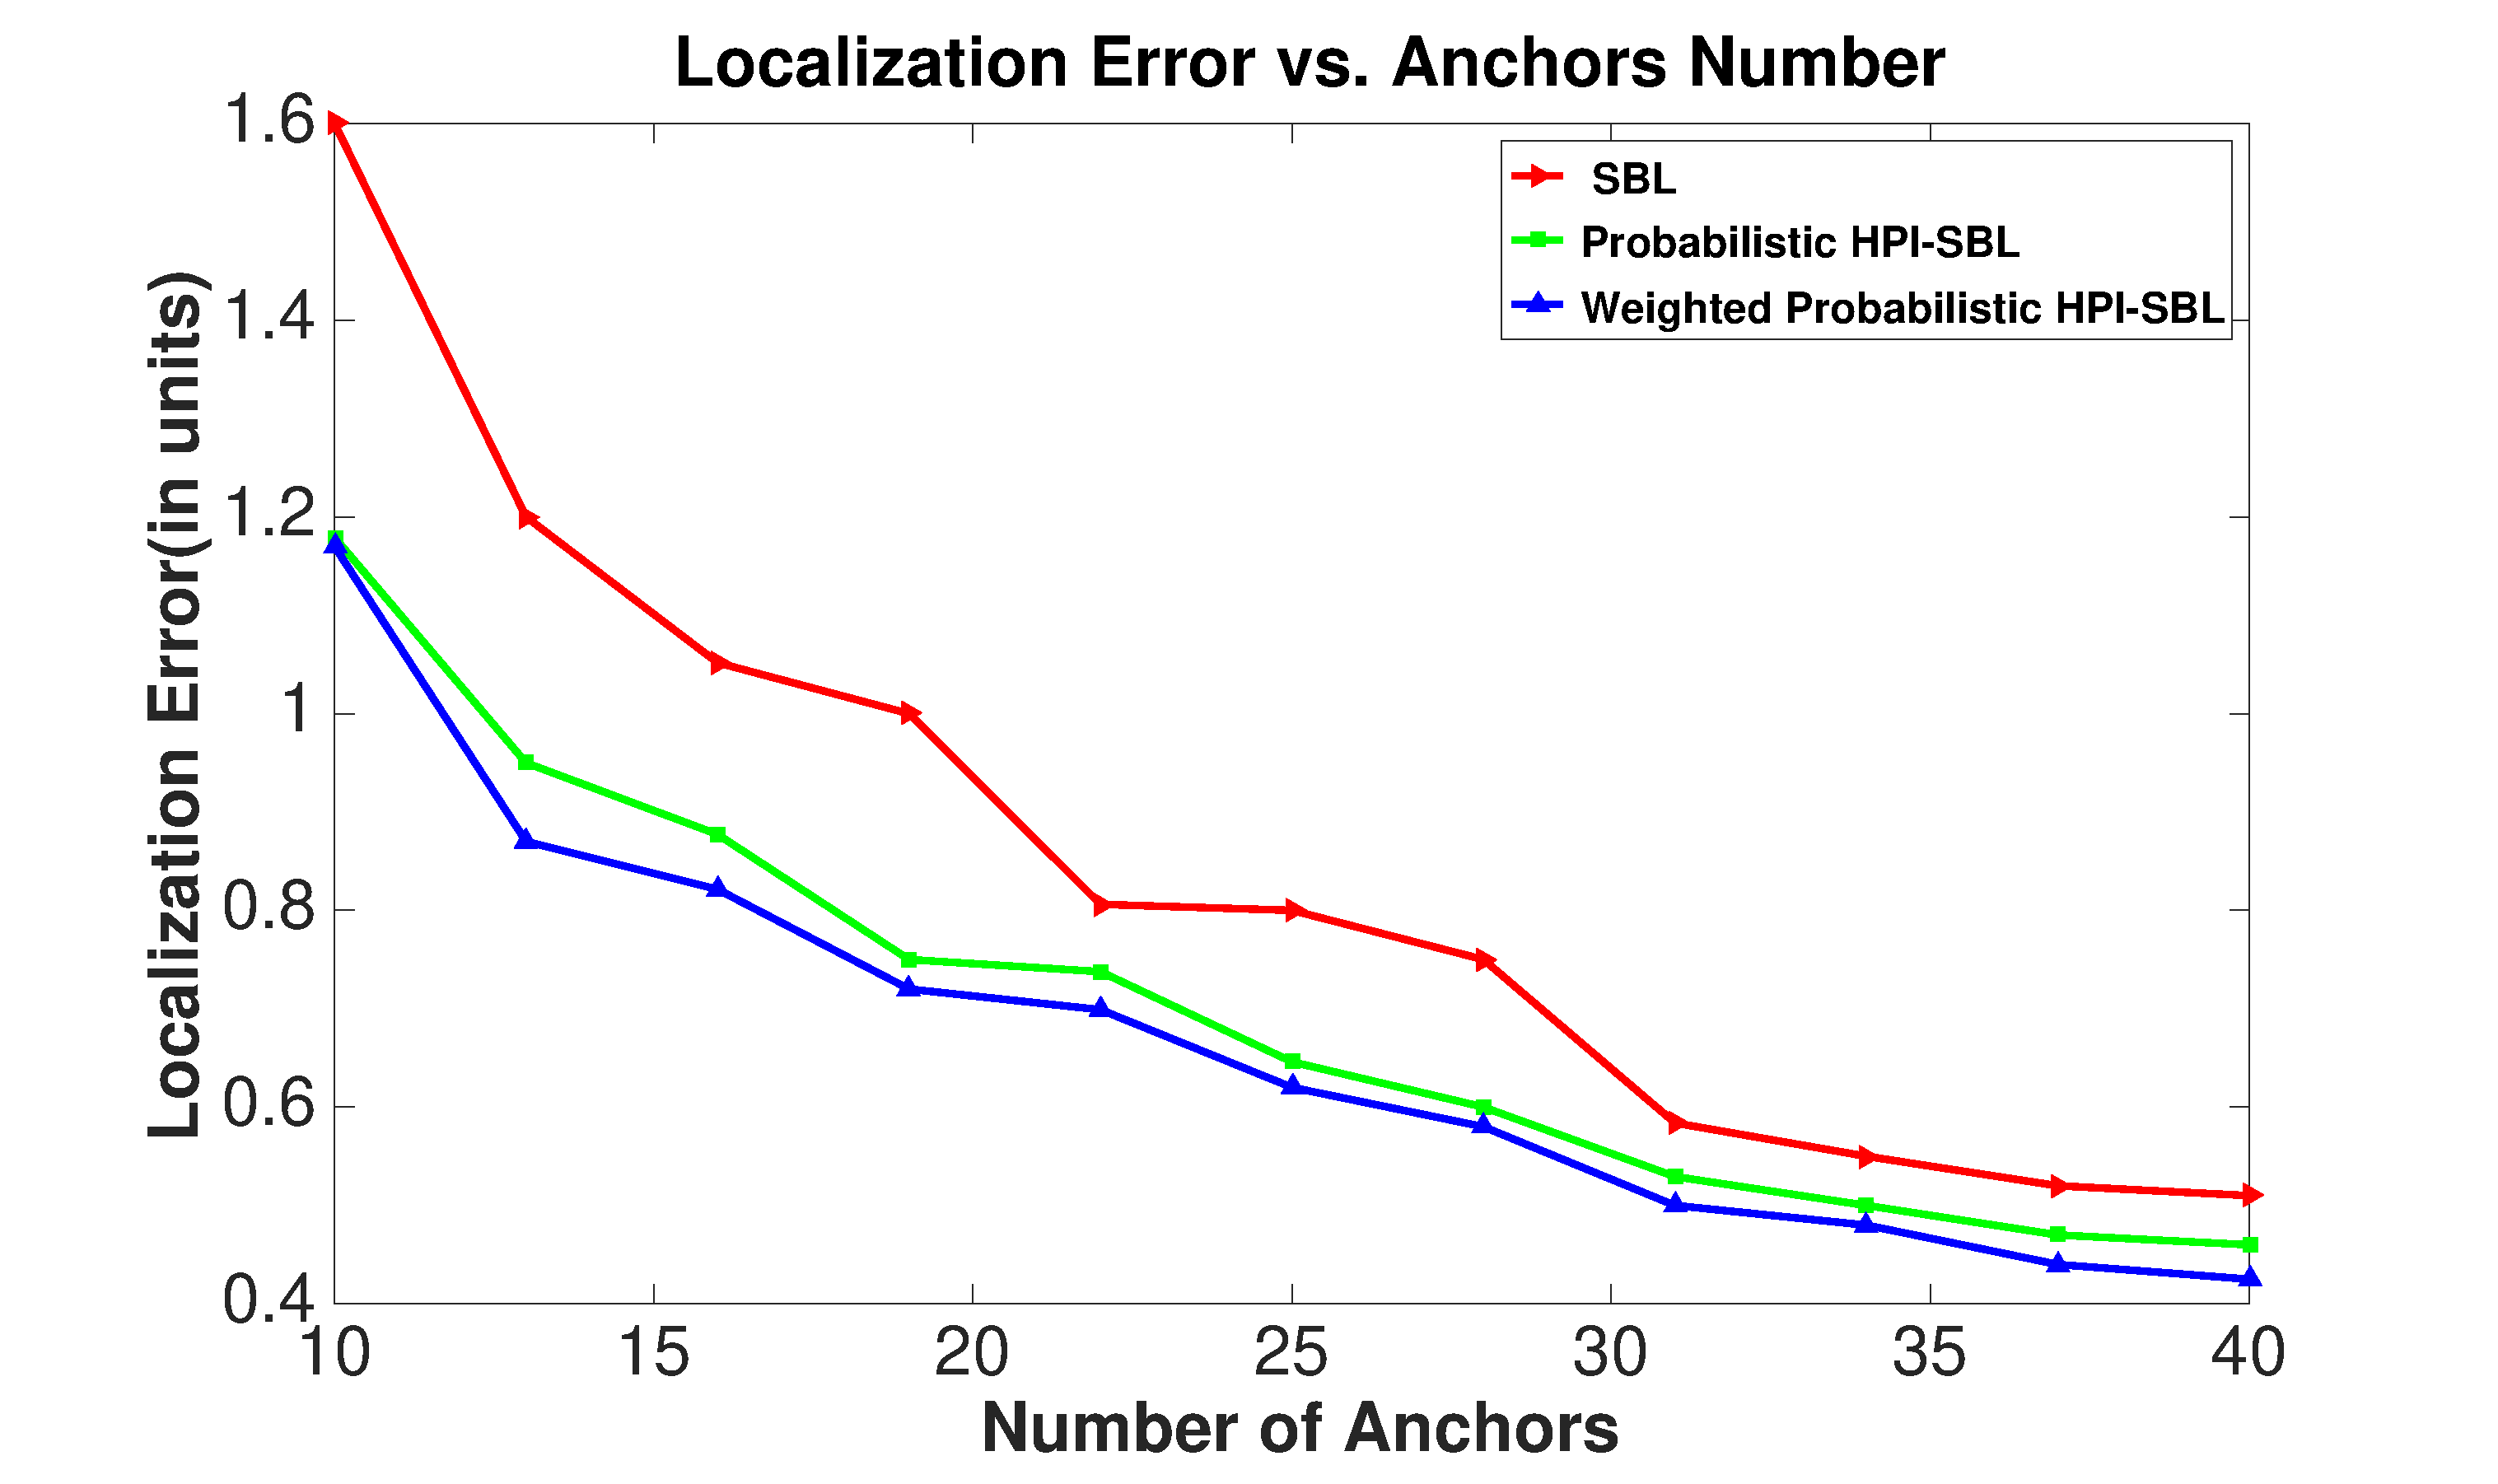
\includegraphics[height=5.0cm,width=7.0cm]{image/nodenumber.eps}
            \caption{Localization Error vs. Number of Anchors}
             \vspace{-5mm}
             \label{fig4}
        \end{figure}

		
\textbf{2) Impact of the location error:}
 %In this experiment, we compared the two methods with different location errors of anchors. 
 We choosed the location error with the range from 0 to 1m in steps of 0.05m for the three methods. 
Fig.\ref{fig5} illustrates a comparison of localization errors between the  SBL and the proposed HPI-SBL.
 Fig.\ref{fig5} indicates the location error of anchors has an effect on the localization results. 
 The proposed HPI-SBL method is more accurate than the SBL method. 
 For the SBL method, the localization error changes obviously as location error increases in Fig.\ref{fig5}. 
 However, as demonstrated in Fig.\ref{fig5}, with the increase location error of nodes, the localization error of HPI-SBL increases relatively slowly, which demonstrates the HPI-SBL method is more robust to the node location error.


  \begin{figure}[htb]
            \centering
		   \vspace{-2mm}
			 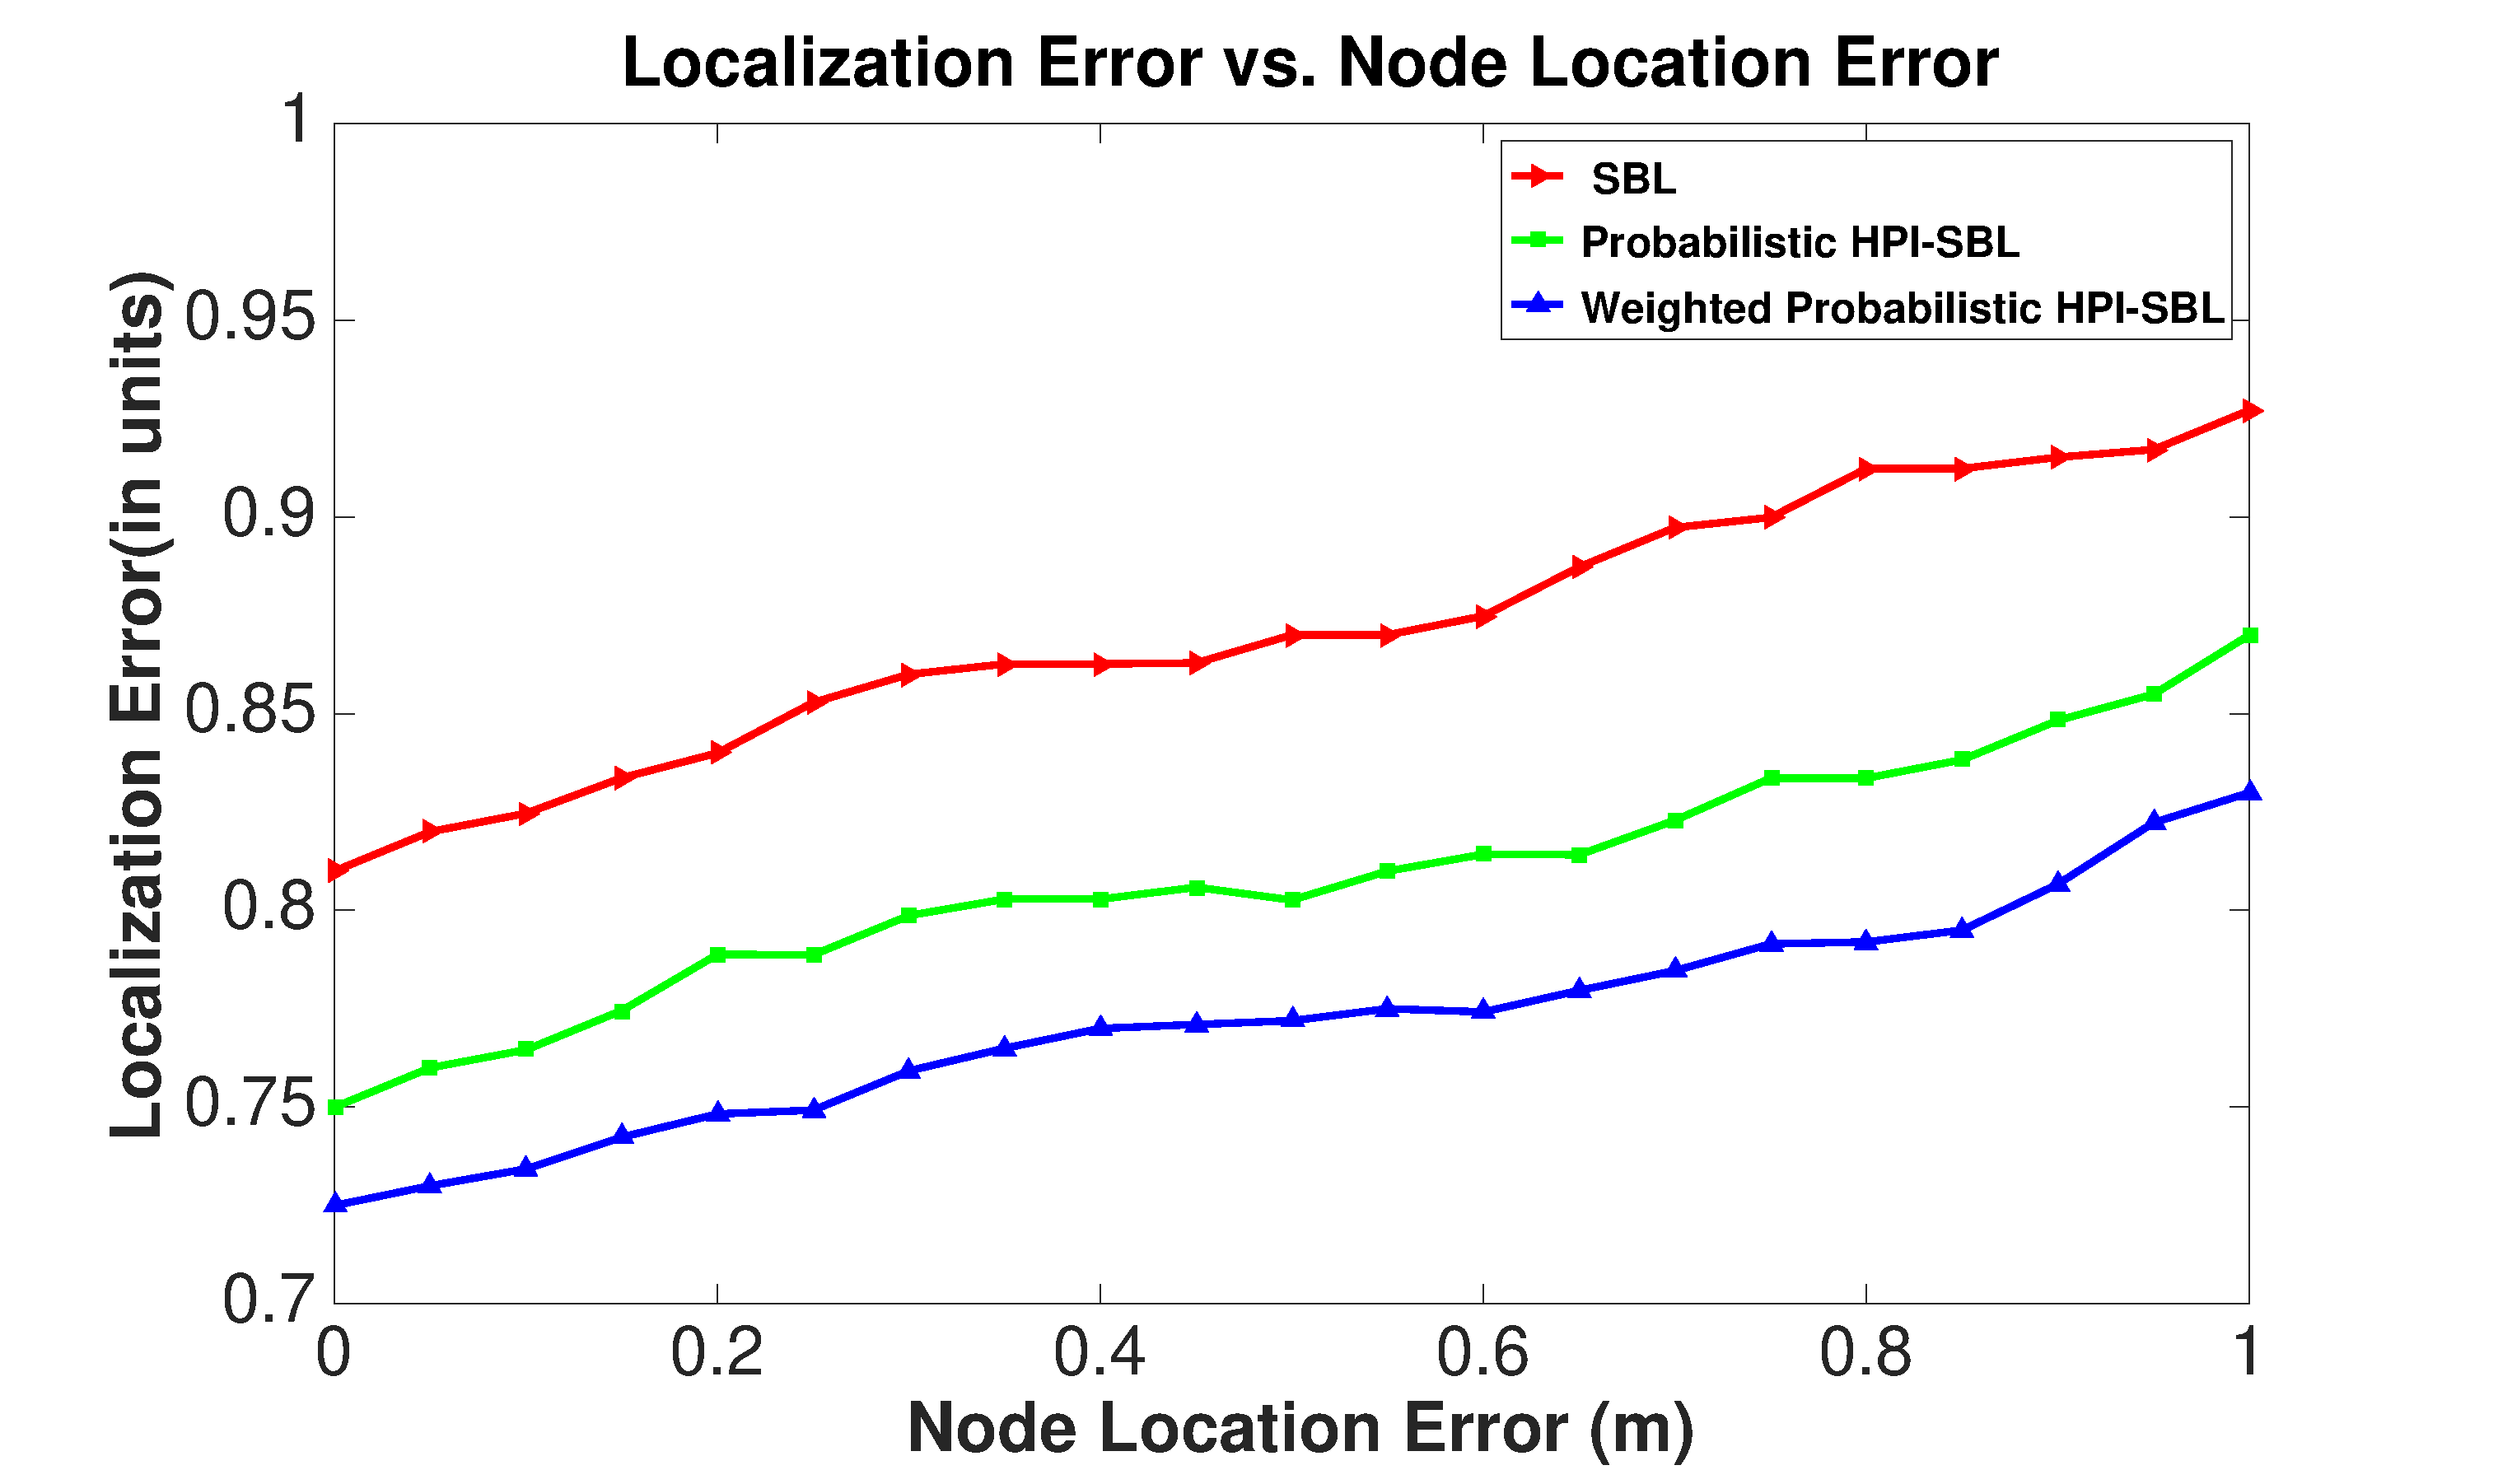
\includegraphics[height=5.0cm,width=7.0cm]{image/location.eps}
            \caption{Localization Error vs. Node Location Error}
             \vspace{-5mm}
             \label{fig5}
        \end{figure}
	

\textbf{3) Impact of the TOA measurement error:}
In this experiment, we performed the impact of the TOA error of anchors for the two methods with the range from 0 to 4ms in steps of 0.25ms. 
Other simulation parameters keep default. 
As it is shown in Fig.\ref{fig6}, the localization errors of the three methods are increasing as the TOA error growth. 
Also, the HPI-SBL method has a better result than the SBL method. We can conclude from this figure that HPI-SBL is more robust to TOA measurement error than SBL.

  \begin{figure}[htb]       
            \centering
			\vspace{-2mm}
            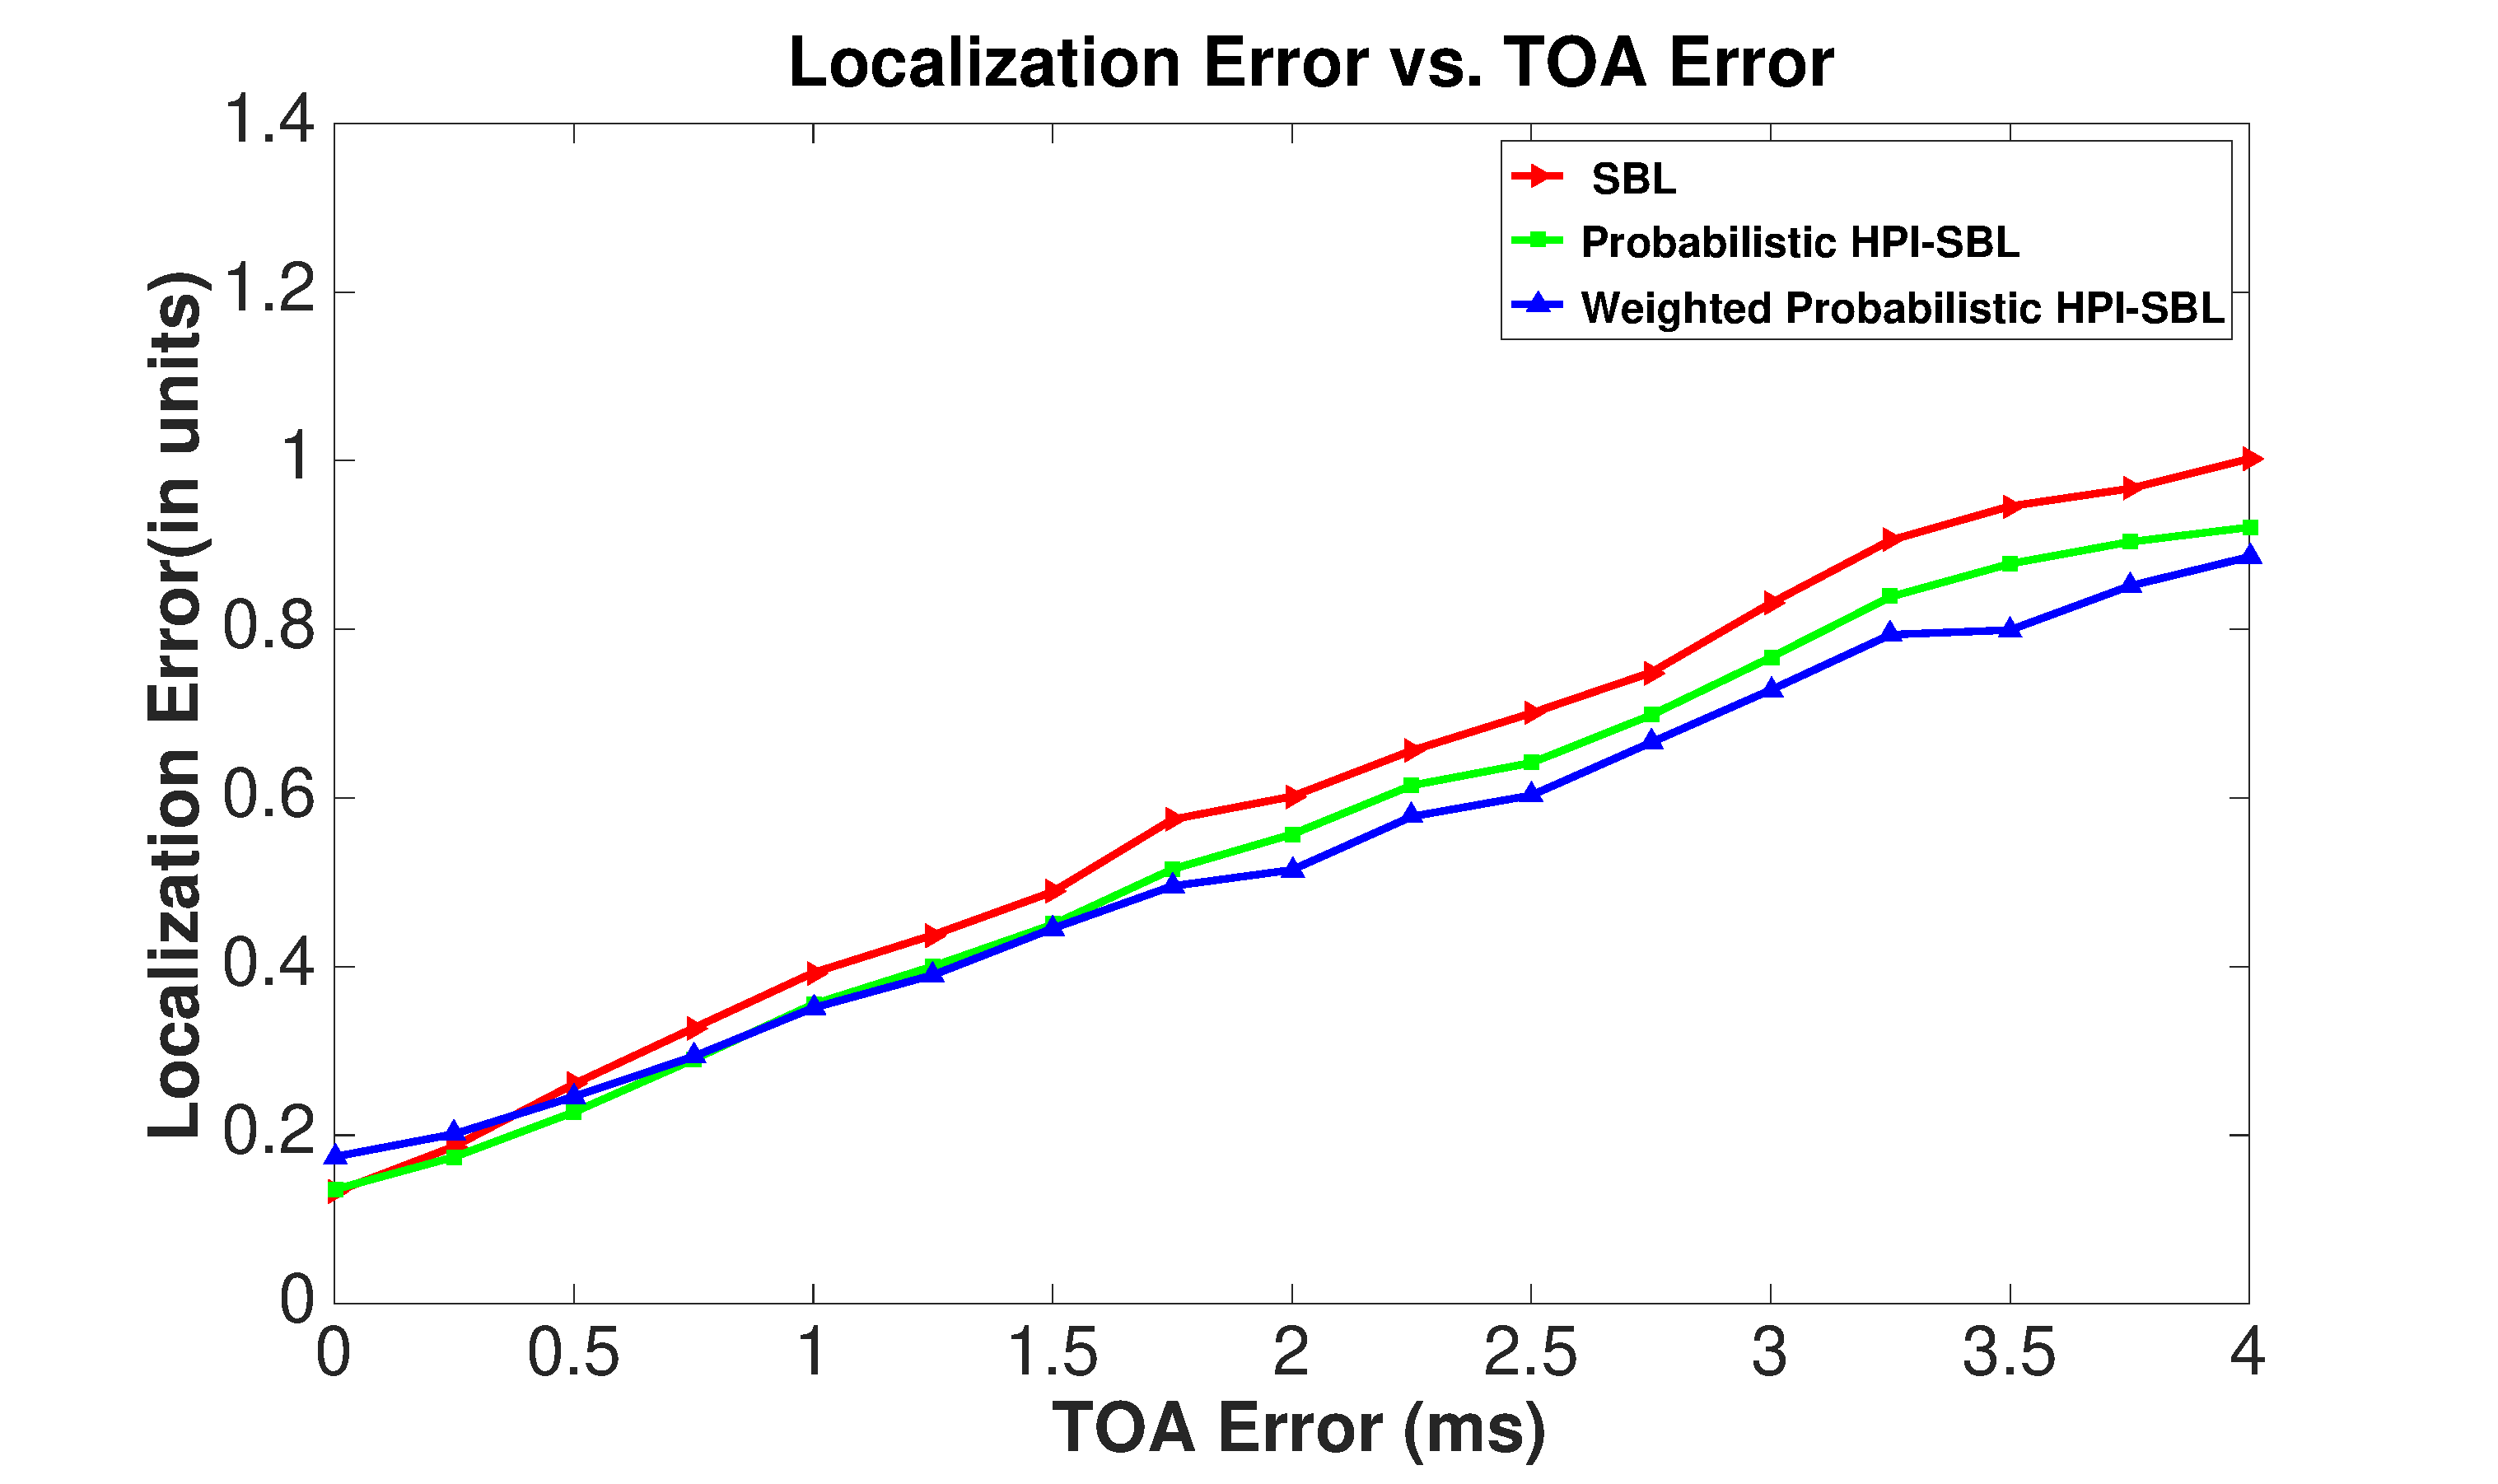
\includegraphics[height=5.0cm,width=7.0cm]{image/TOA.eps}
            \caption{Localization Error vs. TOA Error}
             \vspace{-5mm}
             \label{fig6}
        \end{figure}
		
% \textbf{4) Impact of the probability for P HPI-SBL}
% Time synchronization error maybe also occur flip problem when computing the node sequence in localization system, the impact of time synchronization is similar to TOA measurement error.
% Traditional time synchronization protocol, such as RBS, TPSN, and FTSP, can achieve synchronization with 100ns. 
% Compared with TOA detection error, the effect of time synchronization error is relatively smaller.	
	
  % \begin{figure}[htb]       
            % \centering
			% \vspace{-2mm}
            % 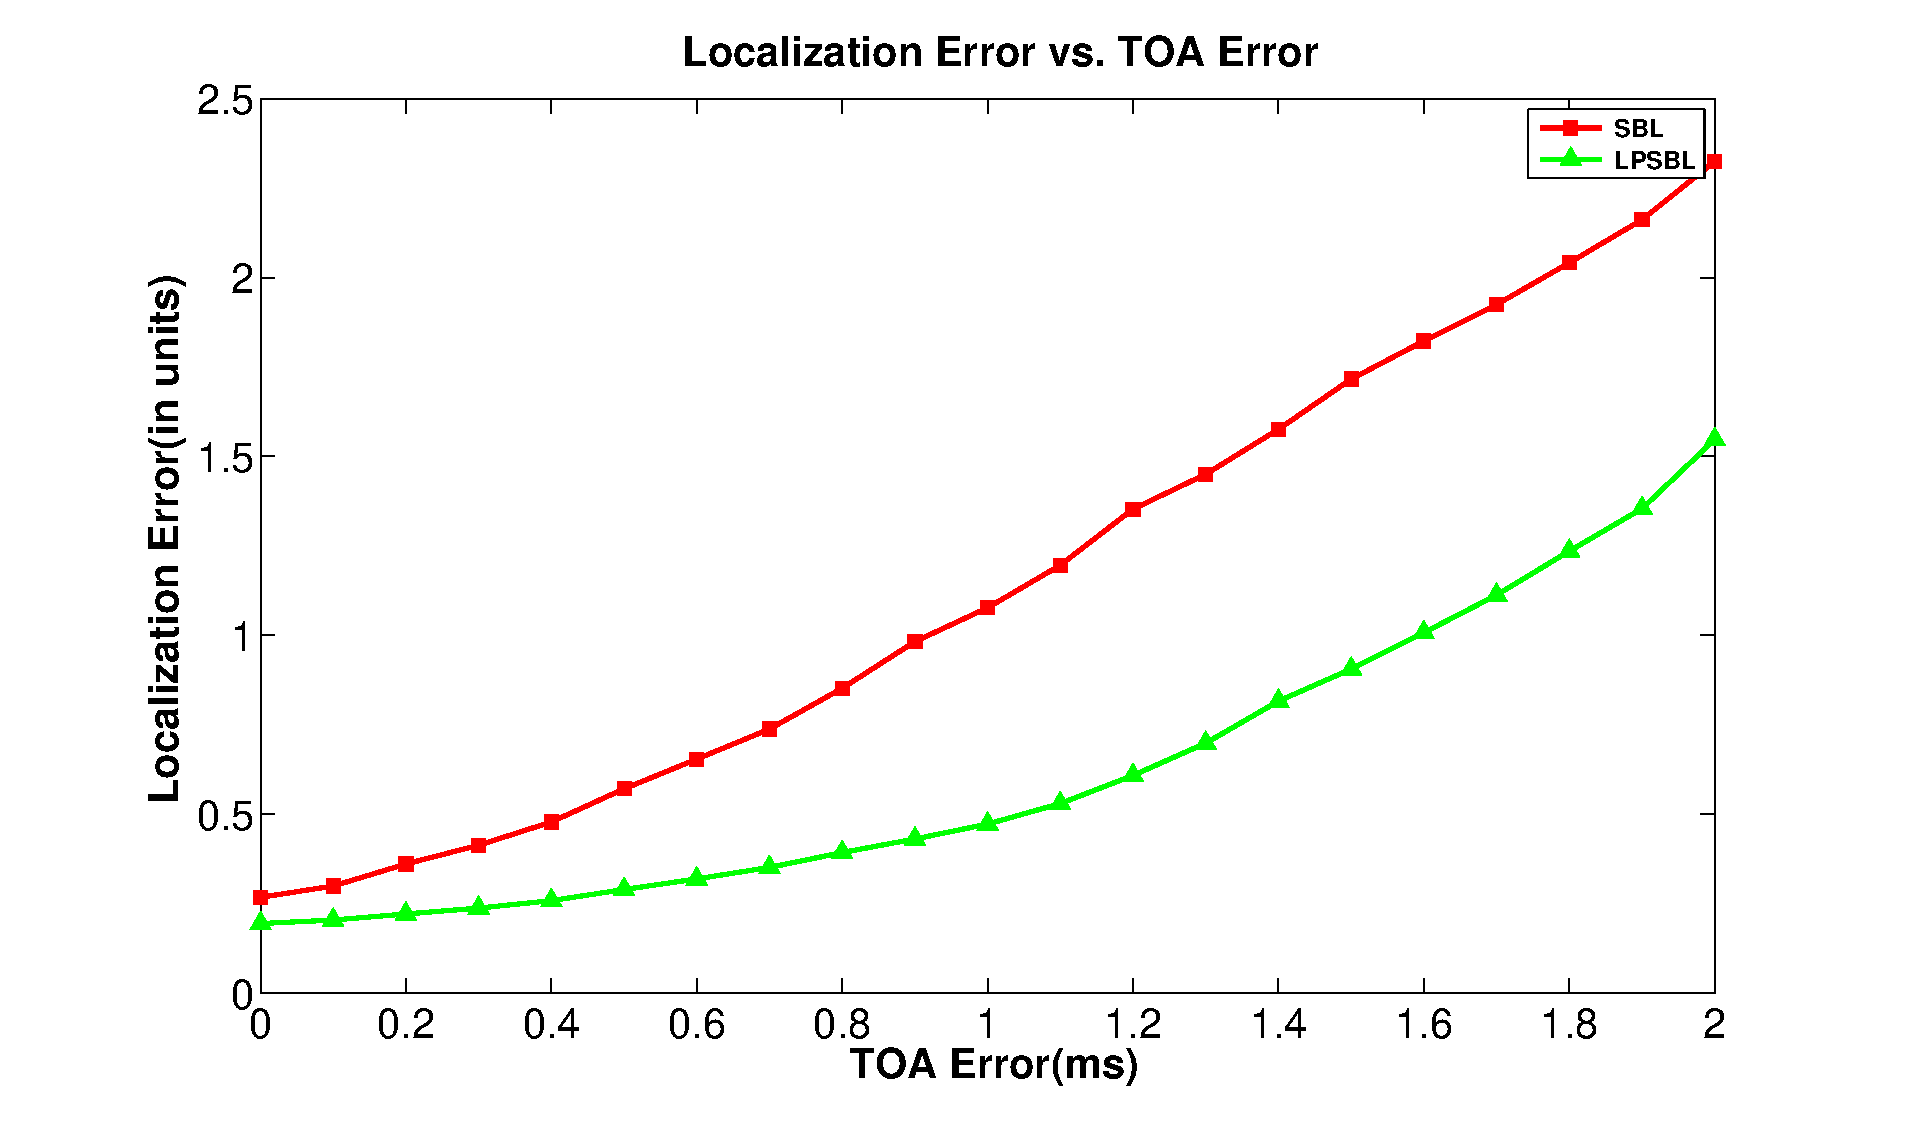
\includegraphics[height=5.0cm,width=7.0cm]{image/fig6.eps}
            % \caption{Localization Error vs. TOA Error}
             % \vspace{-5mm}
             % \label{fig6}
        % \end{figure}



% \textbf{5) Three Weight Scheme P HPI-SBL}

% % 0.5-1   1-0.5   0.5-1-0.5
  % \begin{figure}[htb]       
            % \centering
			% \vspace{-2mm}
            % 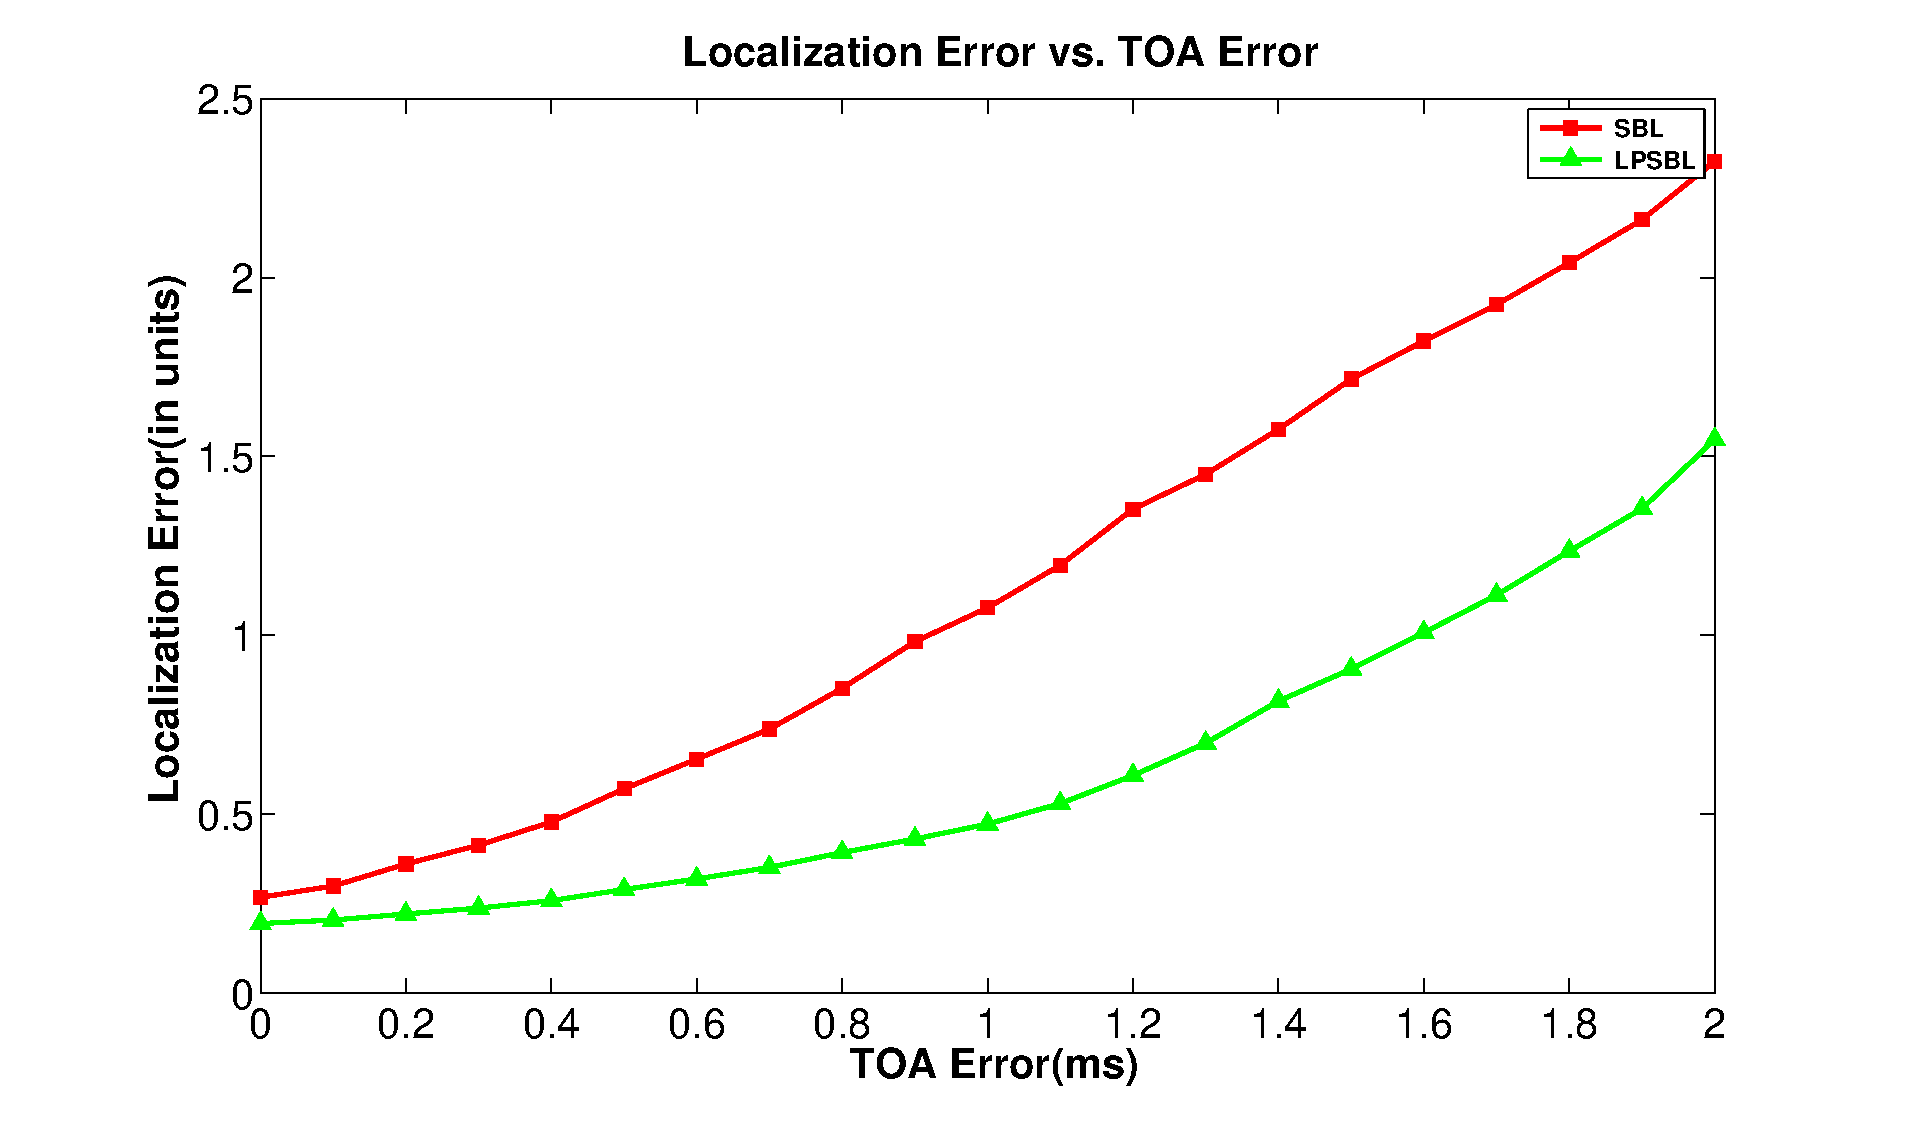
\includegraphics[height=5.0cm,width=7.0cm]{image/fig6.eps}
            % \caption{Localization Error vs. TOA Error}
             % \vspace{-5mm}
             % \label{fig6}
        % \end{figure}

		
 % \textbf{Summary:} From the above simulation results, considering the different factors, 
% including the number of anchors, the node location error and TOA measurement error of the anchors, 
% we can get the conclusion that the proposed HPI-SBL method can achieve better localization performance than SBL method.
% The kernel difference between two methods lies in the way of processing the node sequence.
% By constructing the half-planes from the node sequence, 
% HPI-SBL turns the localization problem into traditional half-plane intersection problem.
% This innovation brings about greatly improved robustness in the localization system.

\subsection{Emulation}


In this section, we reported system implementation of our design based on smartphone arrays.
The 30 smartphones are deployed in a size of 16m$\times$10m space and connected by CISCO CVR328W-K9-CN wireless router.
TPSN protocol is adapted in the proposed HPI-SBL system to realize time synchronization.
In the experiment, smartphones are randomly deployed in the space, and 100 times localization results are shown in Fig.~\ref{fig7}. 
In the figure, blue squares stand for anchor
nodes, red circle squares denote the real position of acoustic sources and black dots are the estimated location by HPI-SBL. 
An arrow origins from the estimated location of each acoustic source and points to its real position. 
As shown in Fig.\ref{fig7}, most of estimated locations are close to the ground truth and the errors between them are very small.
In our experiment, the acoustic sources got localized with average and maximum error of 0.84 feet and 3.91 feet, respectively. Fig.\ref{fig7} tells that
the proposed HPI-SBL successfully accomplishes acoustic source localization with good robustness.


  \begin{figure}[htb]
                  \centering
			    \vspace{-2mm}
            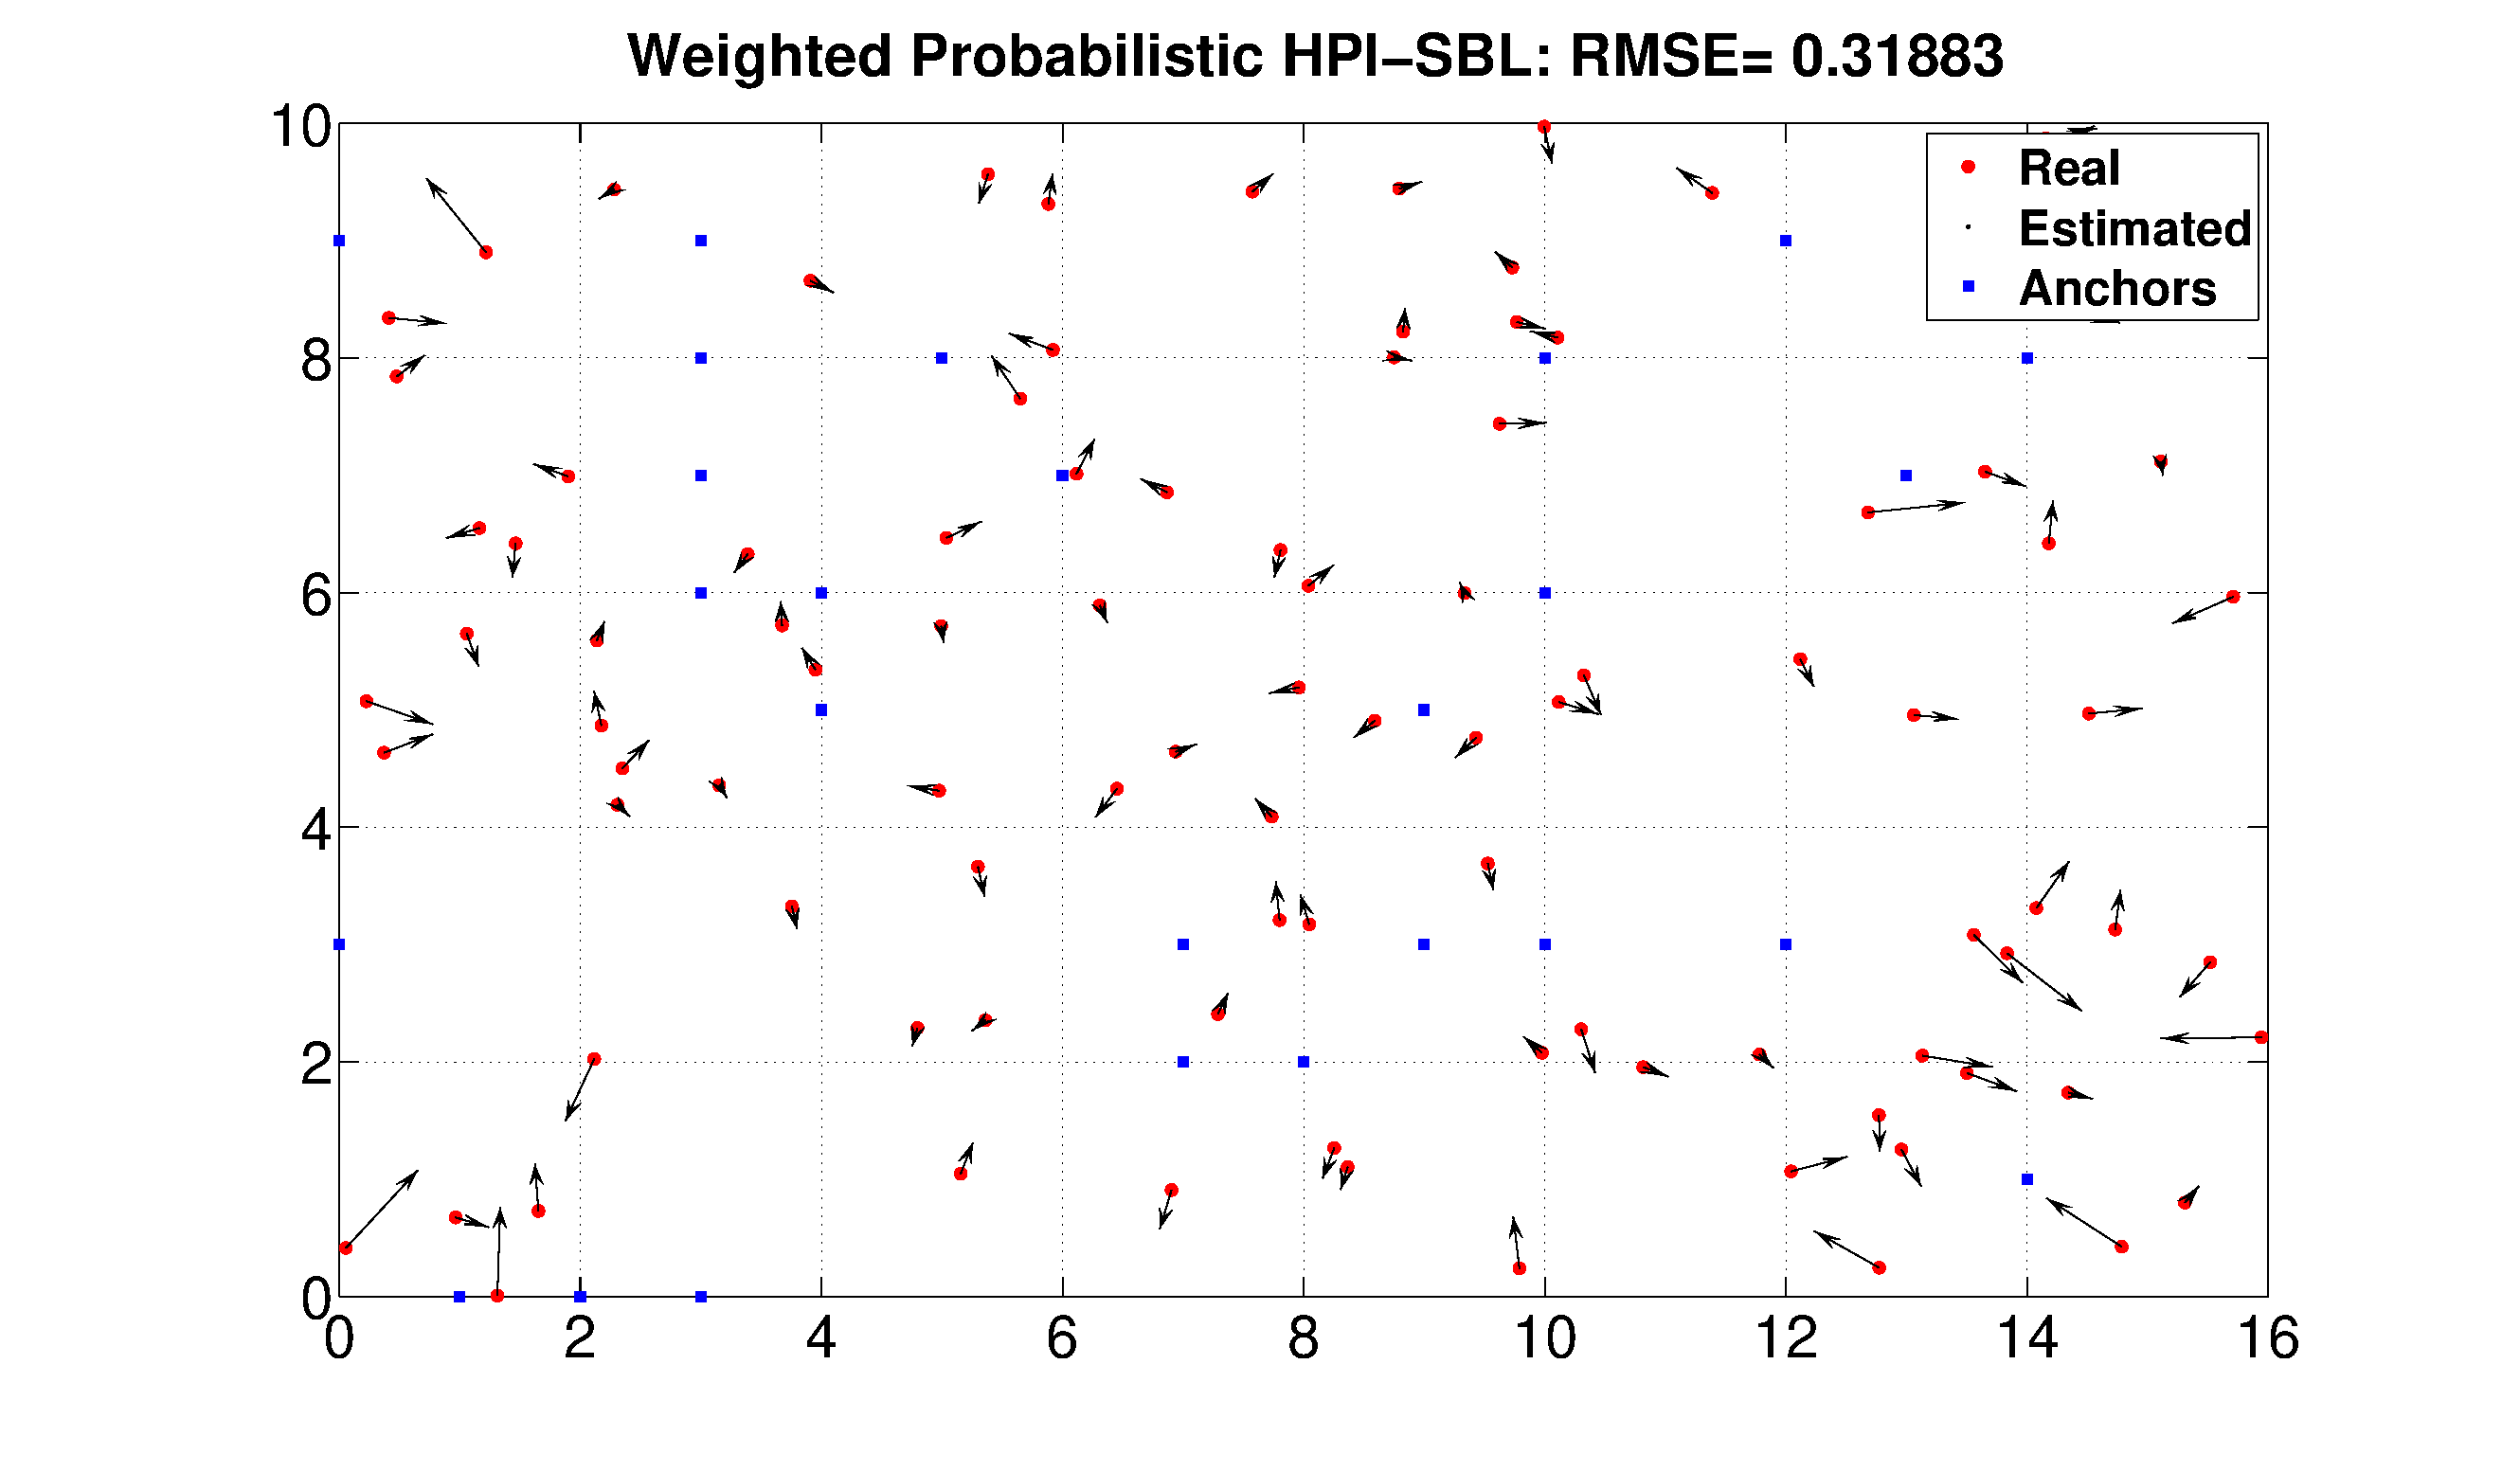
\includegraphics[height=5.0cm,width=7.0cm]{image/testbed.eps}
            \caption{Test-bed localization result of the Weighted Probabilistic HPI-SBL }
             \vspace{-5mm}
             \label{fig7}
        \end{figure}

		
		
\iffalse		
% \begin{figure}[hptb]
% \begin{center}
% \subfigure[Impact of number of anchors]{
% \label{Fig3:3-1}
% \begin{minipage}[t]{0.46\linewidth}
% 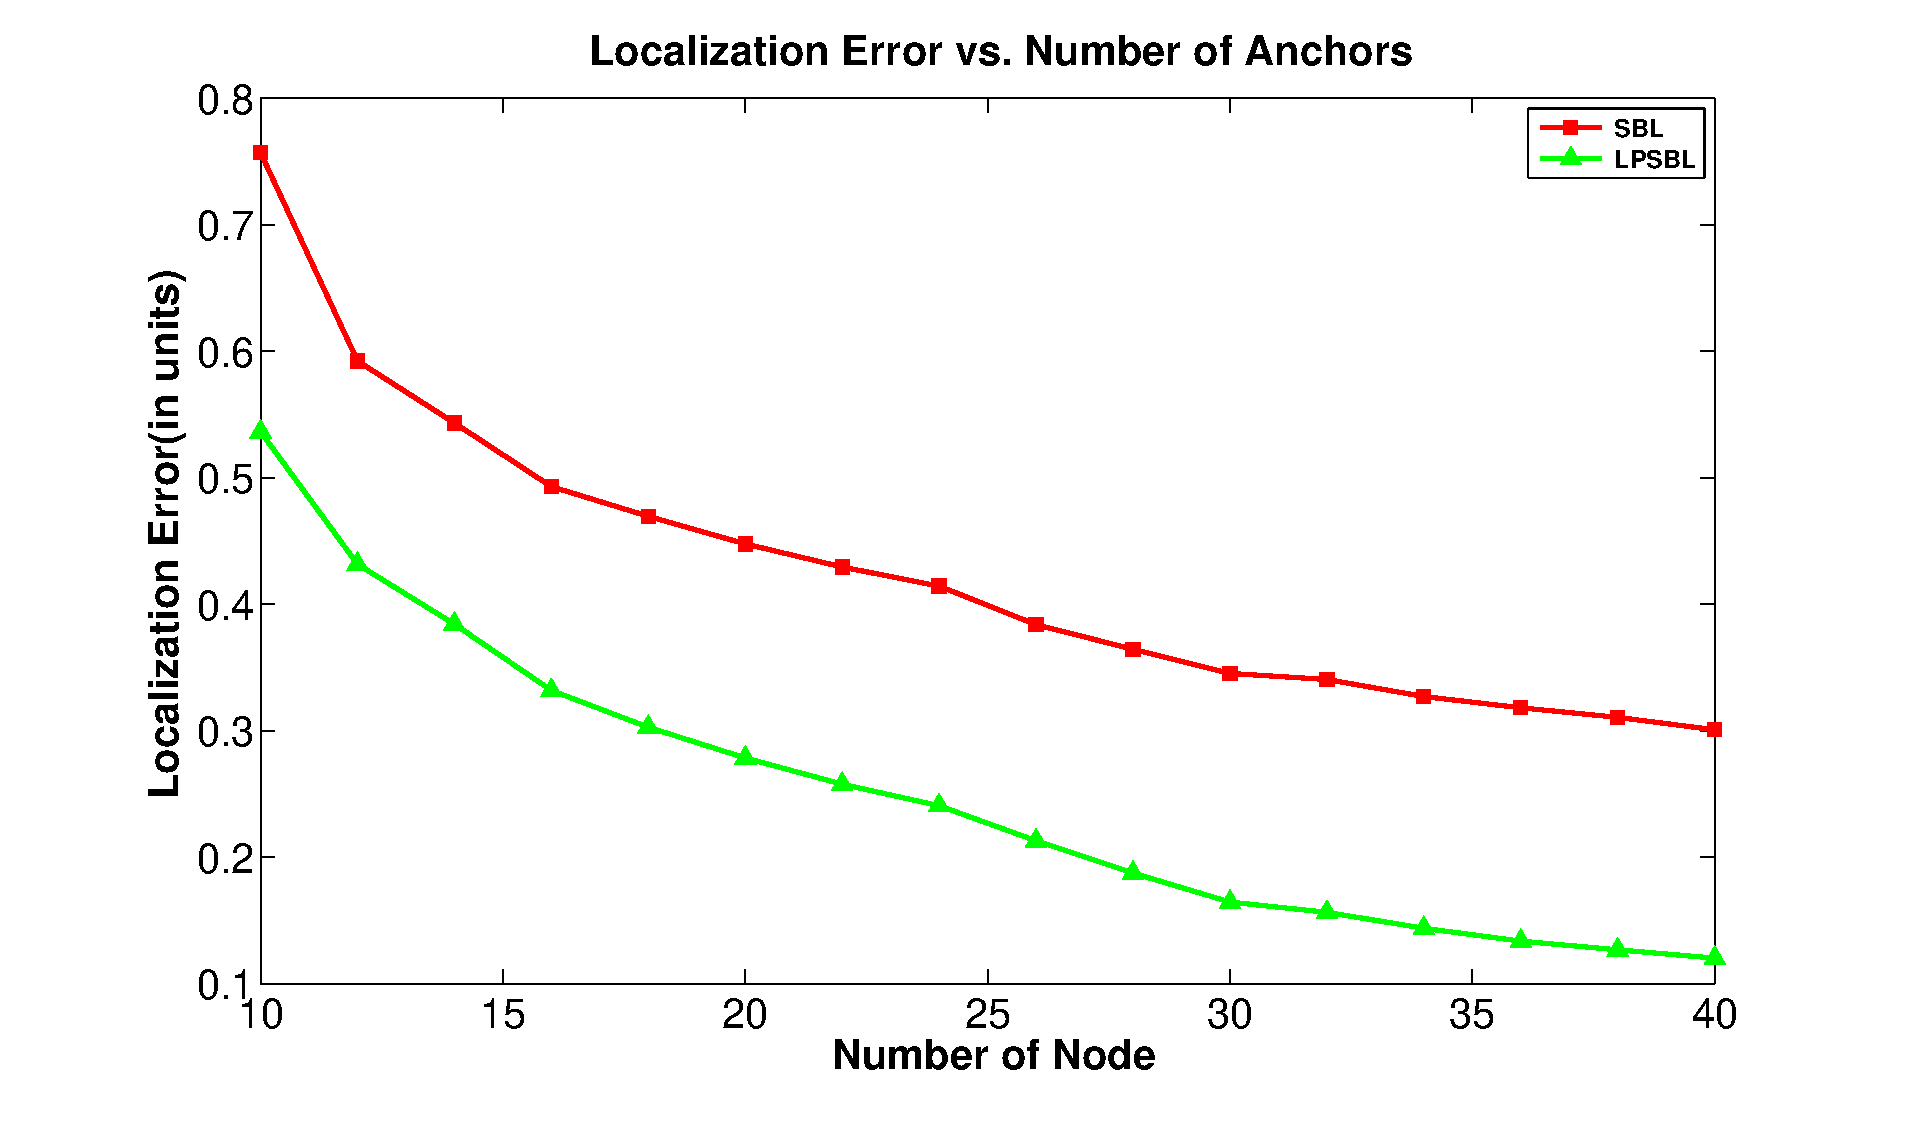
\includegraphics[width=1.150\textwidth]{image/fig4.eps}
% \end{minipage}
% }
% \hspace{-0.1in}
% \subfigure[Impact of node location error]{
% \label{Fig3:3-2}
% \begin{minipage}[t]{0.46\linewidth}
% 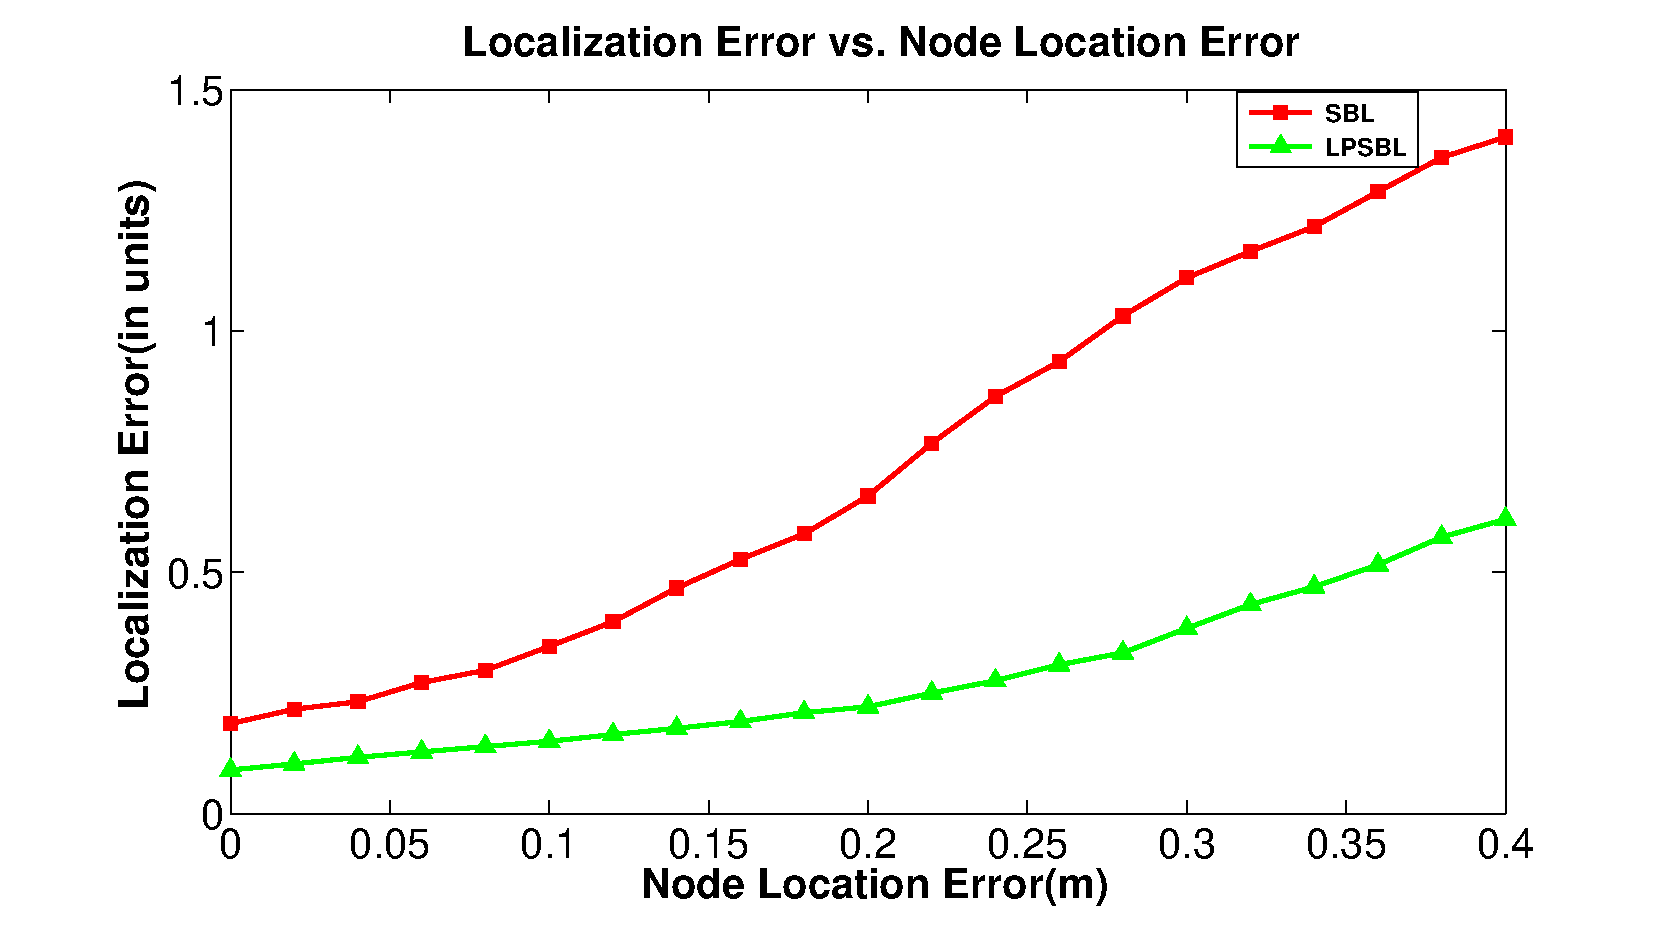
\includegraphics[width=1.150\textwidth]{image/fig5.eps}
% \end{minipage}
% }

% \subfigure[Impact of TOA measurement error]{
% \label{Fig3:3-3}
% \begin{minipage}[t]{0.46\linewidth}
% 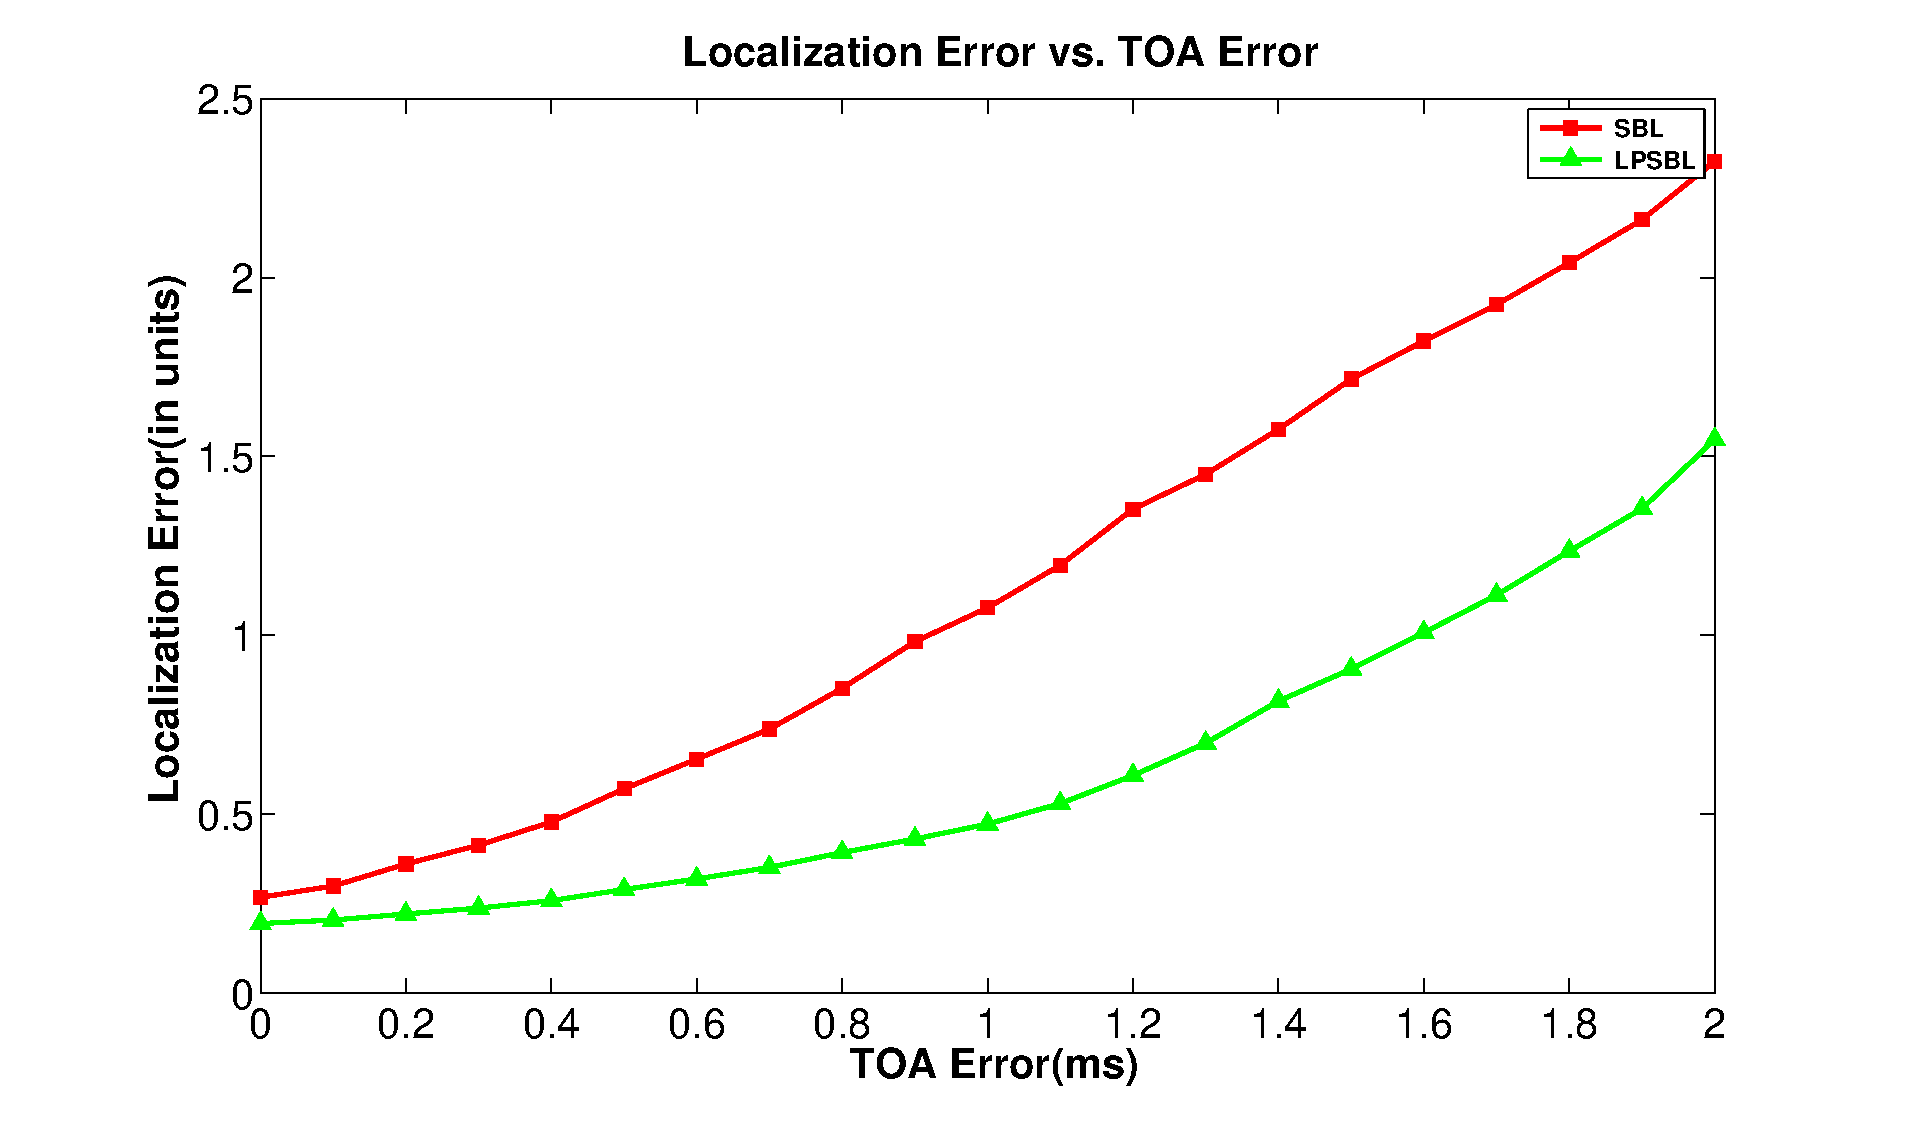
\includegraphics[width=1.150\textwidth]{image/fig6.eps}
% \end{minipage}
% }
% \hspace{-0.1in}
% \subfigure[The results of emulation]{
% \label{Fig3:3-4}
% \begin{minipage}[t]{0.46\linewidth}
% 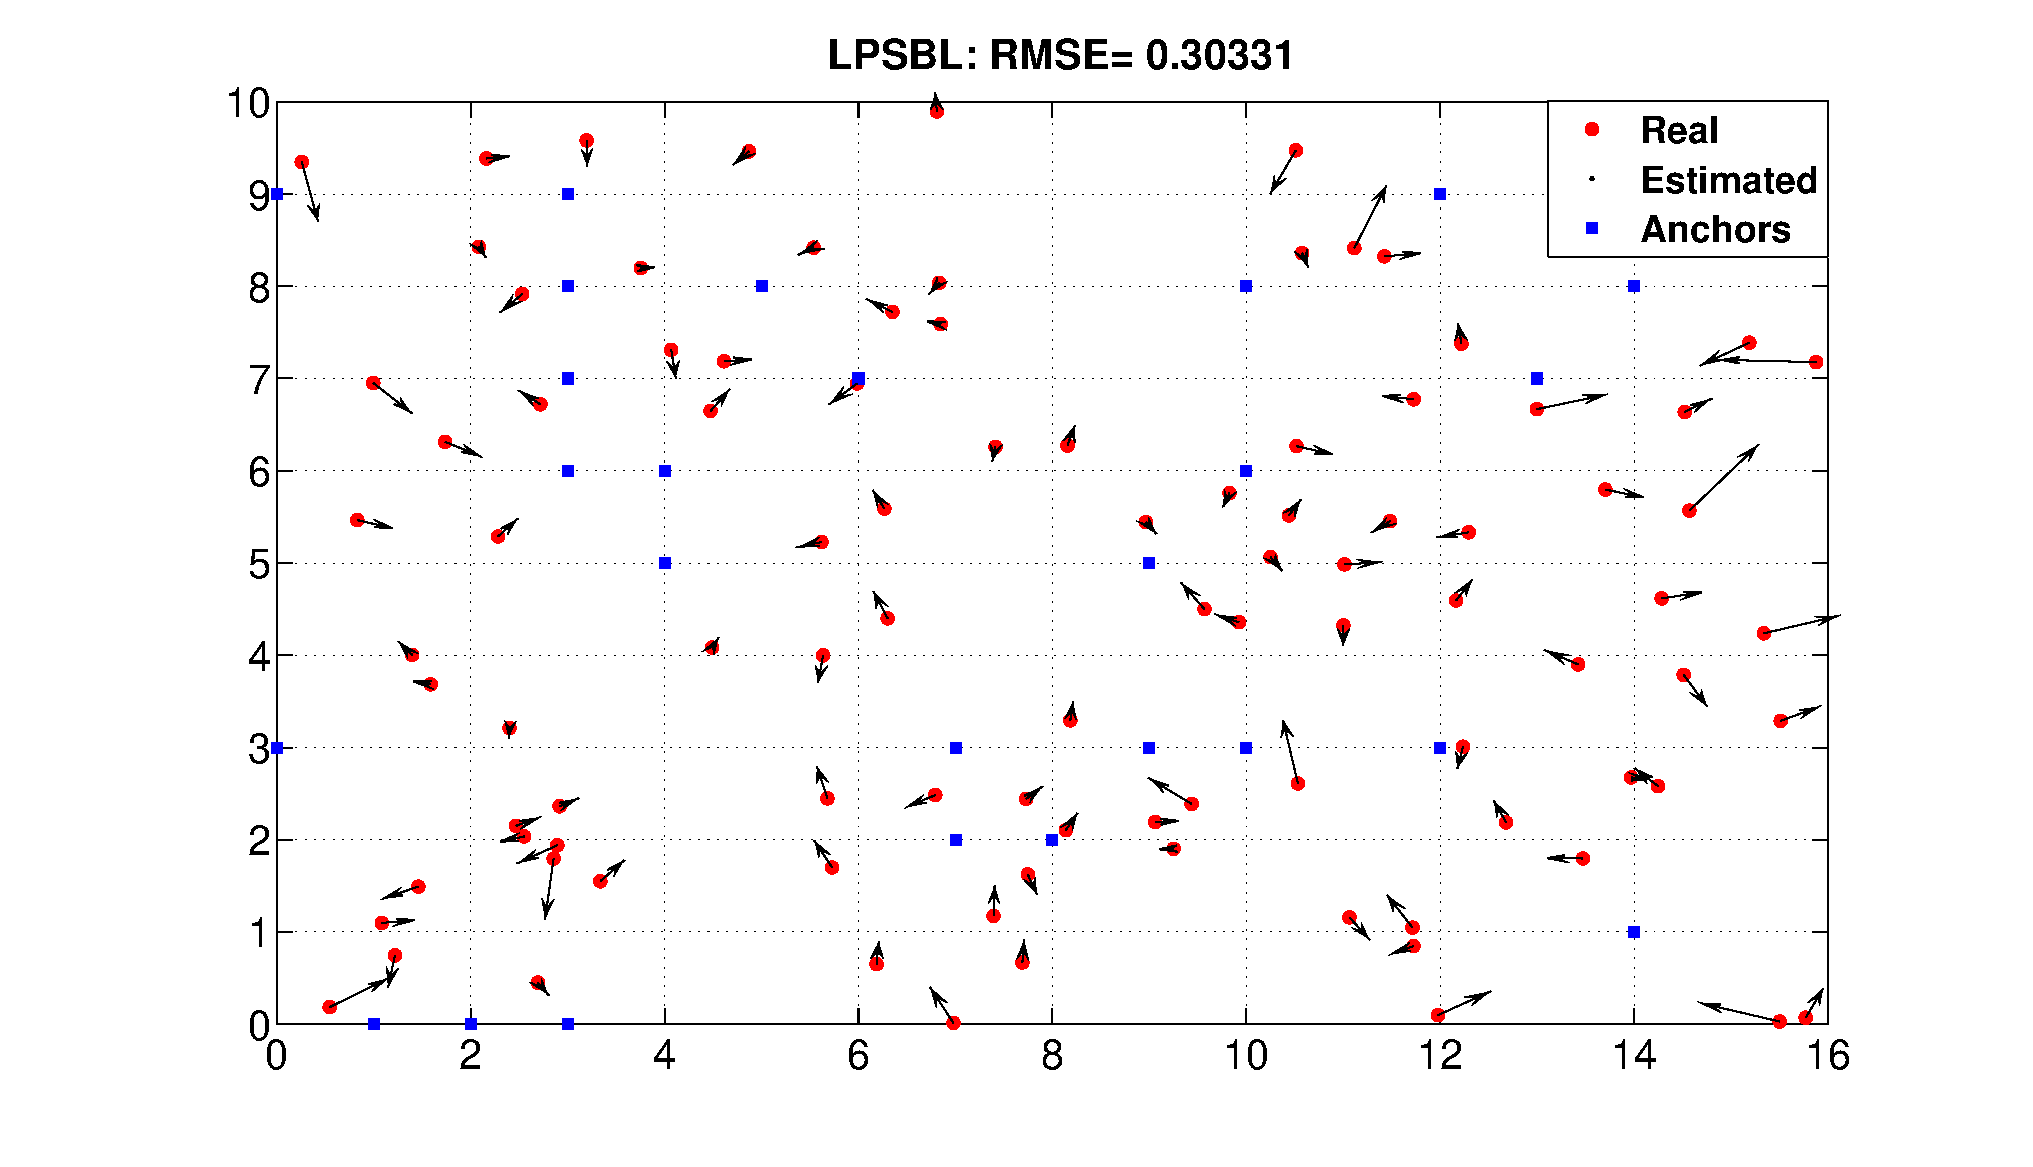
\includegraphics[width=1.150\textwidth]{image/fig7.eps}
% \end{minipage}
% }
% \caption{\label{Fig3:}The results of evaluation.}
% \end{center}
 % \vspace{-5mm}
% \end{figure}
\fi


%%%%%%%%%%%%%%%%%%%%%%%%%%%%%%%%%%%%%%%%%%%%%%%%%

